
\RequirePackage[ngerman=ngerman-x-latest]{hyphsubst}
\documentclass[
        ngerman,
        paper=a4,
        numbers=noendperiod,
]{scrreprt}
\setcounter{secnumdepth}{3}
\setcounter{tocdepth}{3}
% Encoding
\usepackage[utf8]{inputenc}
\usepackage[T1]{fontenc}
% Sprachsupport
\usepackage[ngerman]{babel}
\usepackage{translator}
% Tabellen
\usepackage{booktabs}
\usepackage{tabularx}
\usepackage{pdflscape}
\usepackage{multirow}
% Symbole
\usepackage{eurosym}
% Formeln
\usepackage{amsmath, amsthm, amssymb}
% Formelregeln
\DeclareNewTOC[% 
  counterwithin=chapter, 
  indent=0pt,% kein Einzug im Verzeichnis 
  hang=2em,% Einzug für den Text im Verzeichnis 
  name=equation, 
  type=xequation, 
  nonfloat, 
]{loe} 

\AtBeginDocument{% 
  \newcaptionname{ngerman}\xequationname{Formel}% 
  \newcaptionname{ngerman}\listxequationname{Formelverzeichnis}% 
} 
% Pakete
\usepackage{amsthm}
\usepackage{float}
\usepackage{wrapfig}
\usepackage[babel,german=quotes]{csquotes}
\usepackage[square,sort]{natbib}
\usepackage[hyphens]{url}
\usepackage{setspace}
\onehalfspacing
\usepackage[
        pdftex,
        hyperfigures,
        hyperindex,
        bookmarksnumbered,
        linktoc=all,
        pdfborder={0.25 0.25 0.25},
        %pdfborder={0 0 0},
        pdfpagelayout=TwoColumnRight,
]{hyperref}
\usepackage[all]{hypcap}
\usepackage{lmodern}
\usepackage[final,babel]{microtype}
\usepackage{graphicx}
\usepackage{fancyhdr}
\usepackage[printonlyused]{acronym}
\usepackage{subfiles} 

\pagestyle{fancy}
\renewcommand{\chaptermark}[1]{\markboth{#1}{}}
\fancyhf{}
\fancyhead[RE]{\chaptername~\thechapter}
\fancyhead[LO]{\leftmark}
\fancyhead[LE,RO]{\thepage}

%Quellcodes
%Farben
\usepackage{color}
\definecolor{dkgreen}{rgb}{0,0.6,0}
\definecolor{gray}{rgb}{0.5,0.5,0.5}
\definecolor{mauve}{rgb}{0.58,0,0.82}
%Listing einfaerben
\usepackage{listings}
\lstset{numbers=left,
	numberstyle=\tiny,
	numbersep=5pt,
	breaklines=true,
	showstringspaces=false,
	frame=l ,
	xleftmargin=15pt,
	xrightmargin=15pt,
	basicstyle=\ttfamily\scriptsize,
	stepnumber=1,
	keywordstyle=\color{blue},          % keyword style
  	commentstyle=\color{dkgreen},       % comment style
  	stringstyle=\color{mauve}         % string literal style
}
%Sprache Festelegen
\lstset{language=R}

\begin{document}
\begin{titlepage}
    \begin{center}
    \huge \textbf{\textsf{Implementierung eines QA-Bot-Prototypen aus Wikipedia Zusammenfassungen}} \\
    \vspace{1cm}
    \LARGE\textbf{\textsc{Projektarbeit }}\\
    \vspace{1cm}
    \normalsize
    vorgelegt am: \today \\
    \vspace{2.5cm}
    \large \textbf{Fakultät IV - 
Institut für Wissensbasierte
Systeme und Wissensmanagement, Universität Siegen
}
\linebreak
\linebreak
\begin{figure}[H]
    \centering
\includegraphics[width=0.4\linewidth]{images/imageuni.pdf}
    \label{fig:Unilabel}
\end{figure}
    \end{center}
    \vspace{3cm}
    \begin{center}
 \normalsize{
    \begin{tabular}{ll}
    	Eingereicht von: & {Ugur Tigu} \\
    	Studiengang: & Wirtschaftsinformatik, Master of Science (M.Sc.)\\
	Erstprüfer: & Prof. Dr.-Ing. Madjid Fathi \\
	Betreuer: &   Johannes Zenkert\\
    \end{tabular}\\
    }
\end{center}
\end{titlepage}
\setcounter{page}{0}
\pagenumbering{Roman}
\tableofcontents
\clearpage 
\addcontentsline{toc}{chapter}{Abbildungsverzeichnis}
\listoffigures
\clearpage 
\addcontentsline{toc}{chapter}{Tabellenverzeichnis}
\listoftables
\clearpage 
% Kapiteldefinition ohne Nummerierung
\chapter*{Abkürzungsverzeichnis}
 % Abkürzungsverzeichnis soll im Inhaltsverzeichnis erscheinen
\addcontentsline{toc}{chapter}{Abkürzungsverzeichnis} 
\begin{acronym}
% Format der Abkürzungsdefinition: \acro{}[]{}
% {Verweis}[Abkürzung]{ausgeschriebene Abkürzung}

\acro{nlp}[NLP]{Natural Language Processing}
\acro{qa}[QA]{Question Answering}
\acro{ir}[IR]{Information Retrieval}
\acro{pos}[POS]{Part-of-speech}

\end{acronym}
\clearpage 
\addcontentsline{toc}{chapter}{Formelverzeichnis} 
\listofxequations
\clearpage
\addcontentsline{toc}{chapter}{Listings} 
\lstlistoflistings
\clearpage
\setcounter{page}{1}
\pagenumbering{arabic}











%3 Seiten
\chapter{Einleitung}
\section{Motivation}
\section{Forschungsfragen}
\section{Struktur der Arbeit}




%8 Seiten
\chapter{Theoretische Grundlagen}
\section{Künstliche Intelligenz}
\subsection{Arten von Künstlicher Intelligenz}
\subsection{Geschichte der Künstlichen Intelligenz}
\subsection{Maschinelles Lernen}
\subsection{Künstliches neuronales Netz}

%8 Seiten
\section{Natural Language Processing}
\subsection{Natural Language Processing und Natural Language Understanding}
\subsection{Geschichte des Natural Language Processings}
\subsection{BERT}


%8 Seiten
\section{Question Answering} %2 Seiten
Mit Suchmaschinen wird es den Benutzern immer leichter an gewünschte Informationen heranzukommen. Da Benutzer Schwierigkeiten haben, sich in der Fülle an Informationen der jetzt verfügbaren Online-Informationen zurechtzufinden, wird die Notwendigkeit automatisierter Systeme zur Beantwortung von Fragen immer dringlicher. Wir brauchen Systeme, mit denen ein Benutzer eine Frage in der Alltagssprache stellen und schnell und präzise eine Antwort erhalten kann, mit ausreichendem Kontext. Aktuelle Suchmaschinen können Ranglisten von Dokumenten zurückgeben, liefern dem Benutzer jedoch nicht immer die gewünschten Antworten \citep[S. 275]{Hirschman2001NaturalHere}.

In diesem Kapitel wird das Question Answering in seine einzelnen Elemente zerlegt. Zunächst werden grundlegende Verständnisfragen beantwortet. Was ist Question Answering und Warum gibt es Question Answering?
Es wird eine exemplarische Systemarchitektur vorgestellt, welches alle Elemente des Question Answerings beinhaltet und welche miteinander zusammenarbeiten. 
In den letzten Abschnitten dieses Kapitels wird über die Geschichte, den verschiedenen Paradigmen des Question Answerings und den aktuellen Stand der Forschung berichtet. Dieser Kapitel wird beendet, indem über die Zukunft des Question Answerings und das weitere Potenzial dokumentiert wird.
\subsection{Definitionen der Begriffe}
Um das Question Answering zu verstehen, werden zunächst zunächst
die zugehörigen Begriffe definiert. 

Um eine Frage zu beantworten, muss ein Question Answering System die Frage analysieren, möglicherweise im Zusammenhang mit einer laufenden Interaktion. Es muss eine oder mehrere Antworten finden, indem es Online-Ressourcen konsultiert und es muss dem Benutzer die Antwort in einer geeigneten Form präsentieren, möglicherweise verbunden mit Begründung oder unterstützendem Material \citep[S. 276]{Hirschman2001NaturalHere}. Question Answering Systeme sind Sytsteme, die duch Informationsabruf automatisch Antworten zur gestellten Frage generieren, die Menschen in ihrer natürlichen Sprache stellen. Entweder mithilfe einer vorstrukturierten Datenbank oder einer Sammlung von Dokumenten in natürlicher Sprache \citep{Chali2011ImprovingKernels}\citep{Dwivedi2013ResearchSystem}\citep{Ansari2016IntelligentNetwork}\citep{Lende2016QuestionTechniques}. Es wird dabei abgegrenzt, zwischen \enquote{Fragensatz}, also der gestellten Frage und dem \enquote{Fragentyp}, welches den Zweck einer Kategorisierung der Frage ausweist. In der Literatur bezieht sich der Begriff \enquote{Antworttyp} auf eine Klasse von Objekten, nach denen die Frage sucht. \enquote{Fragenfokus} ist die Eigenschaft oder Entität, nach der die Frage sucht. \enquote{Fragethema} ist das Objekt oder Ereignis, um das es in der Frage geht \citep[S. 2]{CalijorneSoares2018ASystems}. Eine Textpassage welches ein Kandidat für eine Frage ist, wird \enquote{Kandidatenantwort} genannt und ist der Text, der nach seiner Eignung als Antwort eingestuft wird \citep{RetrievalOpen-DomainQuestion-Answering}.

Fragen können nach Antworttyp unterscheiden werden: sachliche Antworten vs. Meinung vs. Zusammenfassung. Obwohl das Verständnis beispielsweise häufig andere Arten von Fragen enthält (Worum geht es in dieser Geschichte? Oder Wie steht der Autor zur Hauptfigur in dieser Geschichte?) konzentriert sich das Question Answering meistens auf Fragen mit sachlichen Antworten. Als nächstes können Fragen nach ihren verschiedene Arten unterscheiden werden: Ja / Nein-Fragen, \enquote{w-Fragen} (Wer war der erste Präsident? Wie viel wiegt ein Wal?), indirekte Abfragen (Liste alle ... auf!) und Befehle (Nennen Sie alle Präsidenten ...). Einige Arten von Fragen sind schwieriger als andere zu beantworten. Zum Beispiel, Warum- und Wie-Fragen, weil sie das Verständnis von Kausalität oder Beziehungen erfordern und diese typischerweise als separate Nebensätze ausgedrückt werden. Die Antworten können lang oder kurz sein, sie können Listen oder Erzählungen sein. Sie können je nach Verwendungszweck variieren. Wenn ein Benutzer beispielsweise eine Begründung wünscht, erfordert dies eine längere Antwort. Es gibt auch verschiedene Methoden zum Erstellen einer Antwort: durch Extrahieren also das Ausschneiden und Einfügen von Ausschnitten aus den Originaldokumenten, die die Antwort enthalten, oder durch Generieren von neuem Text \citep [S. 277-278]{Hirschman2001NaturalHere}. 

Grundsätzlich wird zwischen Faktoiden-, Listen-, Definitions- und komplexe Fragen unterschieden \citep{Kolomiyets2011APerspective}. Faktoide Fragen sind diejenigen, die nach einer einfachen Tatsache fragen und mit wenigen Worten beantwortet werden können, (zum Beispiel: Wie weit ist es von der Erde zum Mars?). Liste Frage fordert als Antwort eine Reihe von Entitäten, die ein bestimmtes Kriterium erfüllen (zum Beispiel: Wann hat Brasilien Fußball Weltmeisterschaften gewonnen? \citep{Heie2012QuestionModelling}. Definitionsfragen erwarten im Gegenzug eine Zusammenfassung oder eine kurze Passage (zum Beispiel: Wie funktioniert die Mitose einer Zelle?) \citep{Neves2015QuestionBiology}. Im Gegensatz dazu handelt es sich bei der komplexen Frage um Informationen in einem Kontext. Normalerweise ist die Antwort eine Zusammenführung von abgerufenen Passagen. Diese Zusammenführung wird mithilfe von Algorithmen implementiert, wie z. B.: Normalisierte Rohbewertung, logistische Regression, Round-Robin, Raw Scoring und 2-Step RSV \citep{Garcia-CumbrerasArchitectureSystem}.


\subsection{Systemarchitektur des Question Answerings} %2 Seiten
Allgemein lässt sich ein Question Answering System in 3 Module unterteilen:
\begin{itemize}
    \item Analyse der Frage
    \item Auswahl geeigneter Dokumente
    \item Verarbeitung der Antwort
\end{itemize}

Der Prozess des Question Answerings geht vom Benutzer aus und das System erhält vom Benutzer eine Eingabe, eine Frage, welches in natürlicher Sprache gestellt wird. Das System soll diese Frage verstehen und dafür findet eine \textit{Analyse der Frage} statt. Die Analyse besteht darin, die Art der Frage herauszufinden, also den Schwerpunkt der Frage oder die Intention zu verstehen \citep{Malik2013DomainSystem}. Die Analyse der vom Nutzer gestellten Fragen wird in zwei Verfahren unterteilt. Das erste Verfahren beschäftigt sich mit der Struktur der Frage, das zweite Verfahren ist es, die Frage so zu transformieren, das Sie mit der QA-Domäne kompatibel ist \citep{Hamed2016AClassification}.

Anders als bei der Analyse der gestellten Frage, wird bei der \textit{Auswahl geeigneter Dokumente} eine Reihe relevanter Dokumente selektiert. Diese dienen als Mögliche Kandidaten für die beantwortung der Frage \cite{Malik2013DomainSystem}. Die abgerufenen Daten können nach ihrer Relevanz für die Frage eingestuft werden \citep{Neves2015QuestionBiology}. 

Die \textit{Verarbeitung der Antwort} ist die schwierigste Aufgabe beim Question Answering. Dieses Modul verwendet Extraktionstechniken. Diese Techniken sollen aus den Dokumenten, die als Kandidaten dienen, eine Antwort presentieren \citep{Bhoir2014QuestionApproach}. Die Antwort muss eine einfache Antwort auf die Frage sein, es kann jedoch erforderlich sein, Informationen aus verschiedenen Quellen zusammenzuführen.

\begin{figure}[H]
    \centering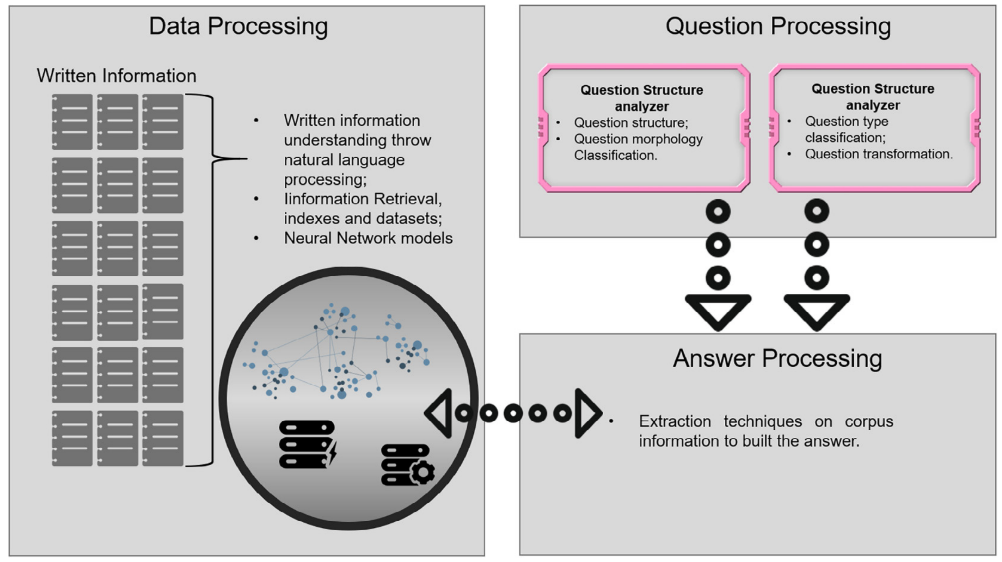
\includegraphics[width=1\linewidth]{images/arch.png}
    \caption[Systemarchitektur]{Allgemeine Systemarchitektur mit 3 Hauptmodulen \cite [S. 3]{CalijorneSoares2018ASystems}}
    \label{fig:architektur}
\end{figure}
\subsection{Geschichte des Question Answerings}
\subsection{Paradigmen des Question Answerings}
\subsection{Stand der Forschung im Question Answering}
\subsection{Zukunft des Question Answerings}

%4 Seiten
\chapter{Technologien und Werkzeuge}
Die im folgenden Kapitel beschriebenen Technologien und Tools werden für die Entwicklung des QA-Chatbot-Prototyps verwendet. Die Beschreibung ist nur oberflächlich. Detaillierte Informationen zur verwendeten Software, zur Systemumgebung und zu den einzelnen installierten Paketen befinden sich in den Anhängen 4 und 5. %todo where
\section{Python}
Python ist eine von der Python Software Foundation weiterentwickelte und veröffentlichte Programmiersprache, die sowohl als objektorientierte Programmiersprache als auch als Skriptsprache angesehen werden kann. Python benötigt relativ wenige Schlüsselwörter, zeichnet sich durch seine Einfachheit, Klarheit und Erweiterbarkeit aus und verfügt über eine große Anzahl wissenschaftlicher Programmbibliotheken auf dem Gebiet Data-Science und wird daher immer mehr zum zentralen Werkzeug. 
Durch so genannte virtuelle Umgebungen, lassen sich die Entwicklungen mittels Python gezielt auf eine Python Version begrenzen und nur bestimmte Pakete mit installieren lassen, somit kann man eine Umgebung für die Softwareverteilung verwenden \citep[S. 2]{GrotzGrundkurs0.1.2d}.
\section{Spacy}
Spacy ist ein Python-Module für die NLP-Entwicklung. Der Fokus liegt dabei auf Geschwindigkeit und Einfachheit. Dabei liefert Spacy die essentiellen NLP-Aufgaben und für jede Aufgabe ist genau ein Algorithmus implementiert worden. Es werden neben Englisch auch Deutsch, Spanisch und Französisch angeboten. Die Annotationen werden dabei in dem Objekt \enquote{doc} gespeichert. Einzelne Wörter werden dabei zu Tokens gemacht. Die Sätze werden automatisch gesplittet und Spacy liefert daneben die Möglichkeit, Named Entity Recognition, den Sentiment, POS-Tagging und viele andere Lösungen für das NLP \citep{SpaCyDocumentation}.

Im Listing 3.1 wird das Modul Spacy mit einem englischen Sprachmodell geladen und eine Frage in der Zeile 2, in seine Tokens zerlegt. Im Anhang wird dazu ein weiteres detailliertes Beispiel im Sinne der Verwendung für diese Arbeit abgebildet.

\begin{lstlisting}[language=Python, caption=Spacy Beispiel]
>>> import spacy
>>> nlp = spacy.load("en_core_web_sm")
>>> question = "What is the capital of Belgium?"
>>> doc = nlp(question)

>>> for token in doc:
>>>   print(token, token.tag_)

# What WP                                    
# is VBZ                                     
# the DT                                     
# capital NN            
# of IN
# Belgium NNP
# ? .

\end{lstlisting}

\section{Transformers}
Transformers (früher bekannt als Pytorch-Transformers und Pytorch-Pretrained-Bert) bieten Allzweckarchitekturen (BERT, GPT-2, RoBERTa, XLM, DistilBert, XLNet) für das Verständnis der natürlichen Sprache (NLU) und die Erzeugung natürlicher Sprachen (NLG). Es bietet über 32 vorgefertigten Modelle und über 100 Natürlichen Sprachen bietet diese Architektur die Interoperabilität zwischen TensorFlow 2.0 und PyTorch.

Das Tokenizer-Objekt ermöglicht die Konvertierung von Zeichenfolgen in Token, die von den verschiedenen Modellen verstanden werden. Jedes Modell verfügt über einen eigenen Tokenizer, und einige Tokenisierungsmethoden unterscheiden sich je nach Tokenizer.

Das Modellobjekt ist eine Modellinstanz, die von einem bestimmten Modul erbt. Jedes Modell wird von seinen Speicher- oder Lademethoden begleitet, entweder aus einer lokalen Datei oder einem lokalen Verzeichnis oder aus einer vorab trainierten Konfiguration. Jedes Modell funktioniert anders und für es wird für eine bestimmte NLP-Aufgabe, ein bestimmtes Modell verwendet \citep{TransformersDocumentation}\citep{PyTorch-TransformersPyTorch}.

\begin{lstlisting}[language=Python, caption=Transformers Beispiel]
>>> from transformers import AutoModelForQuestionAnswering
>>> model = AutoModelForQuestionAnswering.from_pretrained("mrm8488/bert-medium-finetuned-squadv2")
>>> from transformers import AutoTokenizer
>>> tokenizer = AutoTokenizer.from_pretrained("mrm8488/bert-medium-finetuned-squadv2")
\end{lstlisting}

\section{PyTorch}
In diesem Abschnitt wird PyTorch, ein zunehmend beliebtes Python-basiertes Framework für Computergraphen zur Implementierung von Deep-Learning-Algorithmen, dargestellt. Es gibt einen signifikanten Unterschied zwischen PyTorch und anderen Frameworks wie Theano oder Tensorflow. Theano oder Tensorflow folgen grundsätzlich einem \enquote{Definieren-Kompilieren-Ausführen-Paradigma}. PyTorch dagegen ist ein dynamisch definierbares Framework. Es gibt keinen Kompilierungsschritt, der Benutzer kann mathematische Ausdrücke definieren und einen berechennden Operator direkt aufrufen. PyTorch eignet sich somit sehr gut für Forschungszwecke, da es das Entwickeln und Experimentieren mit Deep-Learning-Architekturen relativ einfach ermöglicht \citep[S. 195]{Ketkar2017}.
\section{Wikipedia-Wrapper}
Mit dem Python Modul \enquote{Wikipedia-Wrapper} \citep{Goldsmith/Wikipedia:API} werden  Artikelzusammenfassungen und ganze Wikipedia Artikel erhalten. Der Wikipedia-Wrapper umschließt die MediaWiki-API, sodass Wikipedia Daten verwendet werden können, ohne sie abzurufen.

\begin{quote}
Wikipedia ist die wohl umfangreichste gemeinschaftlich erstellte
Sammlung Freien Wissens in annähernd 300 Sprachen. Allein die
deutschsprachige Ausgabe umfasst weit über zwei Millionen Artikel
– und täglich kommen Hunderte hinzu \citep{WIKIPEDIAWelt}.
\end{quote}

Im Listing 3.3 ist zu sehen, wie durch den Wikipedia-Wrapper, der Inhalt bzw. die Artikelzusammenfassung eines Wikipedia-Artikels in Python erreicht werden kann. Dabei wird im Hintergrund die Wikipedia-API \citep{API:HauptseiteMediaWiki} benutzt.


\begin{lstlisting}[language=Python, caption=Wikipedia Artikelzusammenfassungen]
>>> import wikipedia
>>> print(wikipedia.summary("Question Answering"))
# Question answering (QA) is a computer science discipline within the fields of information retrieval and natural language processing (NLP), which is concerned with building systems that automatically answer questions posed by humans in a natural language.
\end{lstlisting}







\section{Telegram-Wrapper}
Telegram ist eine Messaging-App mit Fokus auf Geschwindigkeit und Sicherheit. Telegram-Bots sind wie kleine Programme, die direkt in Telegram ausgeführt werden. Sie werden von Drittentwicklern mithilfe der Telegram Bot-API erstellt.
Bots sind einfach Telegram-Konten, die von einer Software betrieben werden - nicht von Personen. Sie haben oft KI-Funktionen. Sie können alles tun - lehren, spielen, suchen, senden, erinnern, verbinden, in andere Dienste integrieren oder sogar Befehle an das Internet der Dinge übergeben. Telegram stellt seine API offen für Entwickler zur Verfügung. Telegramm-Bots sind spezielle Konten, für deren Einrichtung keine zusätzliche Telefonnummer erforderlich ist. Diese Konten dienen als Schnittstelle für Code, der auf einem anderen Server ausgeführt wird. Der Vermittlungsserver von Telegram übernimmt für  die gesamte Verschlüsselung und Kommunikation mit der Telegramm-API. Der Nutzer  kommunizieren mit diesem Server über eine einfache HTTPS-Schnittstelle, die eine vereinfachte Version der Telegramm-API bietet \citep{TelegramFAQ}\citep{TelegramAPIs}.

Zusätzlich zur reinen API-Implementierung bietet diese Bibliothek eine Reihe von Klassen auf hoher Ebene, um die Entwicklung von Bots einfach und unkompliziert zu gestalten \citep{Python-telegram-bot/python-telegram-bot:Refuse}.


\section{Flask}
Flask ist ein leichtes Webanwendungsframework. Es wurde entwickelt, um den Einstieg schnell und einfach zu gestalten und um auf komplexe Anwendungen skaliert zu werden. Es begann als einfacher Wrapper um \enquote{Werkzeug} und \enquote{Jinja} und hat sich zu einem der beliebtesten Python-Webanwendungs-Frameworks entwickelt. Es gibt viele Erweiterungen, die von der Community bereitgestellt werden und das Hinzufügen neuer Funktionen vereinfachen.

\begin{lstlisting}[language=Python, caption=Ein einfaches Flask Beispiel]
>>> from flask import Flask

>>> app = Flask(__name__)

>>> @app.route("/")
>>> def hello():
>>>     return "Hello, World!"

$ env FLASK_APP=hello.py flask run

# * Serving Flask app "hello.py"
# * Running on http://127.0.0.1:5000/ (Press CTRL+C to quit)
\end{lstlisting}




%6 Seiten
\chapter{Entwicklung und Implementierung}
In diesem Kapitel werden die wichtigsten Ergebnisse, das Systemverhalten und die Aktionen erläutert, die bei der Entwicklung und Implementierung eines QA-Bots beobachtet wurden. Die in diesem Kapitel erwähnten Beispiele, Verfahren und Szenarien basieren hauptsächlich auf den Beobachtungen, Selbstversuchen und Erfahrungen des Autors, den konkreten Vorschlägen von Expertenkreisen aus Tutorials oder Foren sowie aus der Herstellerdokumentation und den Herstellersoftware-Repositories. Gelegentlich wird auch auf theoretische Ansätze und Grundlagen verwiesen.

Die in diesem Kapitel beschriebenen praktischen Tests und Untersuchungen wurden alle in derselben Systemumgebung durchgeführt. Alle in diesen Unterkapiteln genannten Testergebnisse, Betriebs-, System- und Softwareverhalten sind nur in einer identischen Systemumgebung gültig. Die Hardware-, Betriebssystem- und Softwarespezifikationen der verwendeten Systemumgebung finden Sie in Anhang 4. %todo

Die Verwendung von Python-Befehlen in der Shell für die Ausführung wurde weggelassen. Stattdessen entschied sich der Autor, Python-Skripte zu erstellen und zu verwenden, die die erforderlichen Schritte bündeln und mit einem einzigen Befehl ausführen. Die ausgeführten Befehle werden in den folgenden Unterkapiteln in einem Code-Listing erwähnt. Die verwendeten Skripte befinden sich in den Anhängen 6, 7, 8 und 9. %todo


\section{Entwicklung einer prototypischen Systemarchitektur}


\section{Installation der Software in die Entwicklungsumgebung}
Vor der Installation der Bibliotheken ist eine Python-Umgebung erforderlich, weshalb \enquote{virtualenv} heruntergeladen und installiert wurde. Dieses geschieht mit dem Package Installer für Python \enquote{pip3}.

\begin{lstlisting}[language=bash, caption=Einrichten der virtuellen Umgebung]
$ pip3 install virtualenv
$ virtualenv qabot
$ source qabot/bin/activate
\end{lstlisting}

Wenn die Installationen gut verlaufen sind, ist der nächste Schritt die Installation der erforderlichen Python-Pakete.
Darunter befinden sich auch die  und . Diese Python-Pakete können entweder einzeln per Befehl oder alle zusammen installiert werden, indem sie aus einer Datei gelesen und nacheinander installiert werden. Die Liste der verwendeten Pakete und ihrer Versionen finden Sie in Anhang . Bei der Installation ist darauf zu achten, dass alle Pakete korrekt installiert sind, da viele der Pakete voneinander abhängig sind. Änderungen an Paketversionen können automatisch zu Änderungen an anderen Paketversionen führen, was zu Inkompatibilität führt, da Versionen nicht unterstützt werden. 
Mit \enquote{pip3} werden nun alle Abhängigkeiten für dieses Projekt in die Umgebung installiert.


\begin{lstlisting}[language=bash, caption=Installieren der Abhängigkeiten mit pip3]
$ pip3 install spacy>=2.2.0
$ pip3 install Flask==1.1.2
$ pip3 install python-telegram-bot==12.7
$ pip3 install torch==1.3.1+cpu
$ pip3 install transformers==2.9.1
$ pip3 install wikipedia==1.4.0
\end{lstlisting}



Die erforderlichen Python-Pakete können mit einer Datei zusammengefasst und später in anderen Umgebungen installiert werden, wenn sie in der Datei \enquote{requirements.txt} aufgeführt sind. Um eine require.txt-Datei zu erstellen muss folgender virtualenv Befehl, aus der aktivierten source Umgebung ausgeführt werden:

\begin{lstlisting}[language=bash, caption=Erstellen der requirements.txt Datei]
$ pip3 freeze > requirements.txt
\end{lstlisting}

Somit ist die Entwicklungsumgebung bereit für die Entwicklung.



%3 Seiten
\chapter{Ergebnisse}










%\subfile{Grundlagen/Einleitung}








































\appendix 
\chapter{Anhang}
\label{chapter:Anhang}%


\clearpage
        \phantomsection % damit das pdf bookmark an die richtige Stelle zeigt
        \pdfbookmark{Literaturverzeichnis}{bibliography}
        
        % zeigt immer alle definierten Quellen an, auch wenn diese nicht verwendet werden
        %\nocite{*}
        \bibliographystyle{abbrv}
        \addcontentsline{toc}{chapter}{Literaturverzeichnis}
        \bibliography{literatur}




\chapter*{Erklärung}
Hiermit versichere ich, dass ich die vorliegende Arbeit selbstständig verfasst und keine anderen als die angegebenen Quellen und Hilfsmittel benutzt habe, insbesondere keine anderen als die angegebenen Informationen aus dem Internet. Diejenigen Paragraphen der für mich gültigen Prüfungsordnung, welche etwaige Betrugsversuche betreffen, habe ich zur Kenntnis genommen. Der Speicherung meiner Master-Arbeit zum Zweck der Plagiatsprüfung stimme ich zu. Ich versichere, dass die elektronische Version mit der gedruckten Version inhaltlich übereinstimmt.\newline
\linebreak
\linebreak
\linebreak
Bielefeld, den \today\newline
(Ort) (Datum)\newline
\linebreak
\linebreak
\linebreak
..................................\newline
(Unterschrift)
\end{document}